% Part: sets-functions-relations
% Chapter: relations
% Section: graphs

\documentclass[../../../include/open-logic-section]{subfiles}

\begin{document}

\olfileid[fa-IR]{sfr}{rel}{grp}
\olsection{گراف‌ها}

\emph{گراف} نموداری است که در آن نقطه‌هایی---که «گره» یا «رأس» نامیده
می‌شوند---با یال‌ها به هم متصل‌اند. گراف‌ها ابزاری فراگیر در
ریاضیات گسسته و علوم رایانه‌اند. آنها برای بازنمایی و تجسم روابط و
ساختارها به‌طرزی چشمگیر سودمندند؛ از چیزهای عینی، مانند انواع گوناگون
شبکه‌ها، تا ساختارهای انتزاعی، مانند پیامدهای ممکن تصمیم‌ها. در منابع،
گونه‌های متفاوت بسیاری از گراف‌ها وجود دارند که، برای نمونه، از این
جهت‌ها با هم فرق می‌کنند: یال‌ها جهت‌دارند یا نه، برچسب دارند یا نه،
ممکن است یالی از یک گره به همان گره وجود داشته باشد یا نه، ممکن است
میان همان دو گره چند یال وجود داشته باشد یا نه، و مانند اینها.
\emph{گراف‌های جهت‌دار} پیوندی ویژه با روابط دارند.

\begin{defn}[گراف جهت‌دار]
یک \emph{گراف جهت‌دار} $G = \tuple{V, E}$ از مجموعه‌ای از
\emph{رأس‌ها}~$V$ و مجموعه‌ای از \emph{یال‌ها}~$E \subseteq V^2$
تشکیل می‌شود.
\end{defn}

\begin{explain}
بنا بر تعریف ما، گراف چیزی جز یک مجموعه به‌همراه رابطه‌ای روی آن
مجموعه نیست. البته وقتی از گراف‌ها سخن می‌گوییم، طبیعی است انتظار داشته
باشیم که آنها را به‌صورت تصویری بازنمایی کنند: می‌توانیم گراف را با
کشیدن پیکانی از رأس~$v_1$ به رأس $v_2$ رسم کنیم، اگر و تنها
اگر $\tuple{v_1, v_2} \in E$. تنها تفاوت میان یک رابطه به‌خودی‌خود و
یک گراف این است که گراف مجموعهٔ رأس‌ها را مشخص می‌کند؛ یعنی گراف ممکن
است رأس‌های منزوی داشته باشد. بااین‌حال، نکتهٔ مهم این است که هر
رابطهٔ~$R$ روی مجموعهٔ~$X$ را می‌توان گراف جهت‌دار $\tuple{X, R}$ در
نظر گرفت؛ و برعکس، گراف جهت‌دار~$\tuple{V, E}$ را می‌توان رابطهٔ
$E \subseteq V^2$ دانست که مجموعهٔ $V$ در آن به‌صراحت مشخص شده است.
\end{explain}

\begin{ex}
گراف $\tuple{V, E}$ با $V = \{1, 2, 3, 4\}$ و $E =
\{\tuple{1,1}, \allowbreak \tuple{1, 2}, \allowbreak \tuple{1, 3},
\allowbreak \tuple{2, 3}\}$ چنین شکلی دارد:
\begin{align*}
& 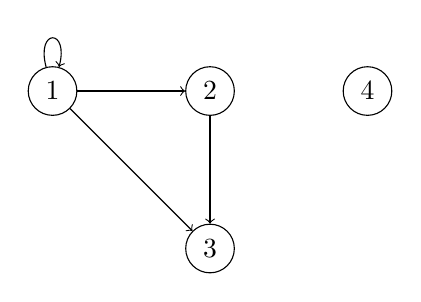
\begin{tikzpicture}[->,node distance=2cm]
  \node[draw,circle] (A) {$1$};
  \node[draw,circle] (B) [right of=A] {$2$};
  \node[draw,circle] (C) [below of=B] {$3$};
  \node[draw,circle] (D) [right of=B] {$4$};
  \draw (A) to [loop above]  (A);
  \draw (A) to  (B);
  \draw (A) to  (C);
  \draw (B) to  (C);
  \end{tikzpicture}
\intertext{این گراف با گراف $\tuple{V', E}$ با $V' =
  \{1, 2, 3\}$ متفاوت است؛ گراف دوم چنین شکلی دارد:}
& 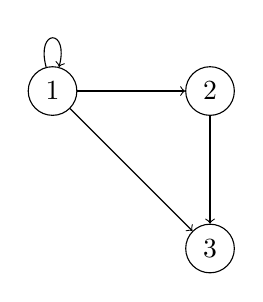
\begin{tikzpicture}[->,node distance=2cm]
  \node[draw,circle] (A) {$1$};
  \node[draw,circle] (B) [right of=A] {$2$};
  \node[draw,circle] (C) [below of=B] {$3$};
  \draw (A) to [loop above]  (A);
  \draw (A) to  (B);
  \draw (A) to  (C);
  \draw (B) to  (C);
  \end{tikzpicture}
\end{align*}
\end{ex}

\begin{prob}
  رابطهٔ کوچک‌تر یا مساوی~$\le$ روی مجموعهٔ $\{1,
  2, 3, 4\}$ را به‌صورت یک گراف در نظر بگیرید و نمودار متناظر را رسم کنید.
\end{prob}

\end{document}
